% !TEX root = thesis.tex
% \chapter{Introduction}
% \label{chap:introduction}

% \section{Context and Motivation}

% \section{Problem Description and Research Questions}

% \section{Research Method}

% \section{Thesis Outline}

\chapter{Introduction}
\label{chap:introduction}

The seas and oceans play a key role in the operation of global ecosystems,
climate
regulation, food security, and energy production~\cite{CopernicusFoodSecurity}.
Monitoring of such large and complex environments requires advanced technology.
Among these, underwater sensor networks (UWSNs) have become valuable resources
for continuous real-time data collection in marine ecosystems, subsea
structures, and oceanic processes~\cite{Domingos2024}.

The SFI Smart Ocean project is designed to create an autonomous and flexible
wireless marine observation program. The system will allow for large-scale,
long-term monitoring of underwater spaces as well as installations by combining
UWSNs and cloud-based big data solutions.
The infrastructure is intended to deal with multi-parameter observations,
ensuring reliable data for both scientific research as well as industrial
applications.~\cite{SmartOceanProject,SmartOceanSite}.

Limitations of acoustic communication, long-range UWSN
deployments are impacted by environmental and
technical challenges.
These consist of power restrictions, minimal data rates and the
inability to recalibrate once deployed at depth. Sensors are subjected to
extreme conditions. Data quality can be affected by pressures, biofouling,
corrosion, along with electronic drift with time. Moreover, environmental
measurements are affected by parameters such as temperature and salinity
can introduce additional uncertainty.~\cite{Skalvik2023}. Once data reaches
surface nodes, there is a need for efficient data handling.
The storage infrastructure needs to be able to deal with large volumes of
inbound data and maintain longterm availability.

The thesis investigates techniques for managing time-series data produced by
the Smart Ocean sensor network. The emphasis is on evaluating the development
of database technologies that can deal with large-scale storage and effective
querying of time-stamped observations. The work contributes to the wider
picture of the Smart Ocean which aims to promote data-driven decision making in
marine operations. This research aligns with the ACM Computing Classification
System (CCS) under Information systems → Data management systems → Database
administration → Database performance evaluation~\cite{ACM-CCS-2012}. The study
focuses on
evaluating and comparing time-series database technologies to improve the
efficiency and reliability of underwater sensor data management.

% \newpage
\section{Context and Motivation}
% SmartOceanSite
\subsection{The SFI Smart Ocean Platform}
% The SFI Smart Ocean initiative, funded by the Norwegian Research Council, is a
% collaborative effort between research institutions and industry partners
% focusing on key challenges in developing smart ocean systems
% ~\cite{SmartOceanSite}. The initiative concentrates on three primary areas:
The Norwegian Research Council has provided funding for the SFI Smart Ocean
project.
Research institutes as well as industry partners work together on key issues in
building smart ocean systems~\cite{SmartOceanHub}. The initiative concentrates
on 3 main areas:

\begin{enumerate}
      \item \textbf{Underwater Sensor and Measurement Technology}: Focuses on
            developing autonomous sensors and methods for real-time monitoring
            of underwater environments. These sensors include features like
            data
            collection, acoustic communication, and energy-efficient
            operations.

      \item \textbf{Underwater Wireless Sensor Networks Based on Acoustic
                  Communication}: Addresses the establishment of reliable
            communication networks for data transmission from underwater
            sensors.

      \item \textbf{Smart Ocean Platform for Cloud-Based Data and Application
                  Services}: Consists of developing the Smart Ocean platform to
            incorporate, process, and visualize ocean information. The platform
            uses Standard APIs \& efficiently formats to deal with data from
            diverse underwater sensors.
\end{enumerate}

\newpage
\subsection{Motivation}
The deployment of Smart Ocean's sensor network will generate a large volume of
time series data. The underwater sensors continuously measure parameters over
extended periods, resulting in a continuous stream of timestamped readings. The
data volume rapidly reaches big-data scales with dozens or possibly hundreds of
sensors reporting in real time (each measuring several variables).
The system needs to store years of data reliably, deal with high-frequency
ingestion, and support queries for real-time alerts and long-term analysis a
major challenge.

The selection of suitable data management technologies is crucial given these
requirements. Standard relational databases, although robust, are
not specifically designed to deal with high-volume time-series workloads
where data arrives sequentially and is mainly queried by time. In recent years,
specialized Time-Series Management Systems (TSMSs) have emerged in response to
the high-volume, high-velocity nature of data generated by IoT devices and
sensors. Unlike general-purpose databases, TSMSs are architected to efficiently
store, query, and process time-stamped data streams, making them uniquely
suited for real-time sensor workloads~\cite{Jensen2017}. This systems are
designed to efficiently ingest and index time-stamped data
and provide built-in functions for time-window queries, downsampling, and
time-centric analytics. Dedicated TSDBs are increasingly considered a natural
fit for fast sensor data streams, yet with a wide variety of database options
available, it is not obvious which technology is most suitable for the Smart
Ocean platform.

\newpage
\section{Problem Description and Research Questions}
the best way to efficiently store and manage
the large amounts of time-series data generated by the Smart Ocean platform in
the above mentioned context is to determine what database
technology (or combination of technologies) best meets the platform's demands
for scalability, functionality as well as dependability in dealing with
underwater sensor data. It involves comparing various approaches. For example
traditional relational databases with time-series extensions versus
purpose-built
time-series databases to figure out their relative advantages and disadvantages
for Smart Ocean's use case.

The investigation is guided by the following research question and
sub-questions:

\begin{itemize}
      \item \textbf{Main Research Question:} \emph{Which database technology is
                  most suitable for managing large-scale time-series data
                  % from the
                  % SFI Smart Ocean platform, and why?
            }
      \item \textbf{RQ1:} What are the key requirements and challenges in
            managing
            % Smart Ocean’s time-series 
            sensor data (e.g., data volume, frequency of
            data, query patterns, real-time access needs, and deployment
            constraints)?
      \item \textbf{RQ2:} Which existing database systems
            (relational, NoSQL, and dedicated time-series databases)
            are potential candidates for this task, and what are their
            expected advantages or limitations in the Smart Ocean context?
      \item \textbf{RQ3:} How do selected candidate databases perform
            % under representative Smart Ocean data workloads in terms of data
            ingestion rate, query performance, scalability, storage efficiency,
            and other relevant metrics?
\end{itemize}

\newpage
\section{Research Method}
To answer the research questions, this thesis applies the evaluation
methodology proposed by Brown and Wallnau~\cite{Brown1996}.
Their framework provides a structured way to assess software technologies
through the definition of measurable benchmarks or technology deltas, that
highlight how one technology performs relative to another. The methodology is
organized into three phases: descriptive modeling, experiment design, and
experiment evaluation. Figure~\ref{fig:framework} illustrates the overall
structure of this framework.

The descriptive modeling phase consists of identifying the relevant features.
This involves determining which requirements are most relevant for evaluation.
These requirements then form the basis for defining performance benchmarks such
as ingestion throughput, query latency, scalability, and storage efficiency.

The experiment design phase serves as the planning stage of the evaluation.
In this phase, hypotheses are formulated about how different database
technologies are expected to behave under representative workloads. Workload
models and test harnesses are developed to simulate large-scale time-series
data, ensuring that the experiments are both realistic and repeatable.

Finally, in the experiment evaluation phase, the selected databases are tested
using the defined benchmarks. The resulting measurements are
collected, analyzed, and compared to highlight the deltas between technologies.
This process enables a systematic assessment of strengths, weaknesses, and
trade-offs, ultimately guiding conclusions about which database technologies
are most suitable for handling time-series data at scale.

\begin{figure}
      \centering
      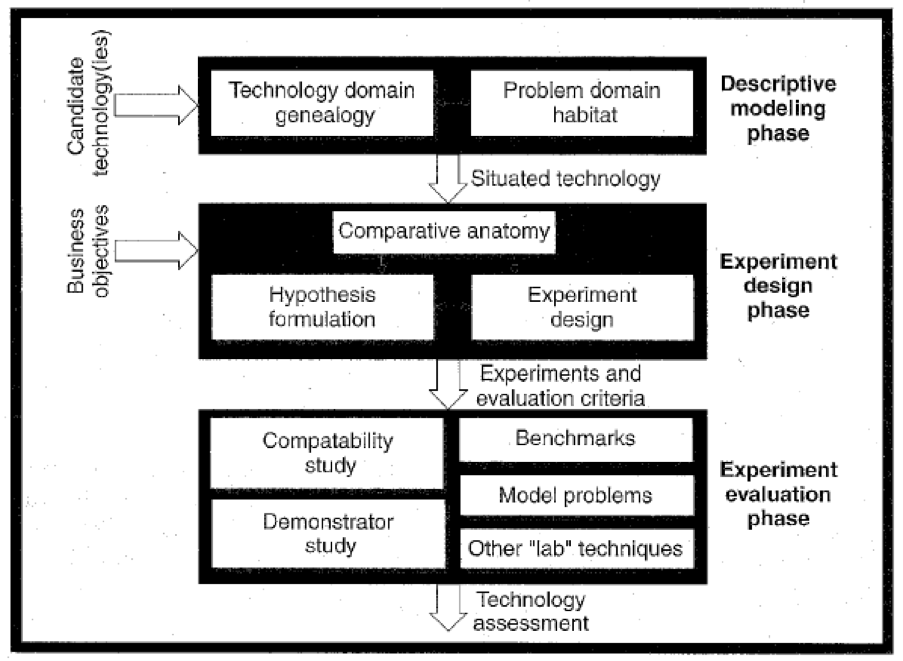
\includegraphics[scale=0.8]{figs/framework.png}
      \caption{Software technology evaluation framework.}
      \label{fig:framework}
\end{figure}

\newpage
\section{Thesis Outline}
The remainder of this thesis is organized as follows:

\begin{itemize}
      \item \textbf{Chapter 2 – Background and Related Work:} Provides the
            necessary background
            and
            context. Reviews time-series data characteristics and challenges,
            and
            surveys existing database technologies for time-series data
            management.
            Discusses related work and prior evaluations of database
            performance
            in
            IoT and sensor data scenarios.
      \item \textbf{Chapter 3 – Design and Analysis:} Outlines the design of
            the
            experimental evaluation, including the selection of database
            technologies, the design of test workloads, and the metrics used
            for assessment.
      \item \textbf{Chapter 4 – Implementation and Prototypes:} Describes the
            implementation of the experimental setup, including the deployment
            of database systems and the creation of test environments. Details
            the development of prototypes or models used for evaluation.
      \item \textbf{Chapter 5 – Evaluation and Results:} Presents the empirical
            results of the
            comparative evaluation of database technologies. Includes ingestion
            throughput, query performance, storage efficiency, and other
            findings.
      \item \textbf{Chapter 6 – Conclusion and Future Work:} Summarizes key
            findings and
            contributions, provides recommendations for the Smart Ocean
            platform,
            and
            suggests directions for future work.
\end{itemize}
